\documentclass{beamer}\usepackage[]{graphicx}\usepackage[]{color}
%% maxwidth is the original width if it is less than linewidth
%% otherwise use linewidth (to make sure the graphics do not exceed the margin)
\makeatletter
\def\maxwidth{ %
  \ifdim\Gin@nat@width>\linewidth
    \linewidth
  \else
    \Gin@nat@width
  \fi
}
\makeatother

\definecolor{fgcolor}{rgb}{0.345, 0.345, 0.345}
\newcommand{\hlnum}[1]{\textcolor[rgb]{0.686,0.059,0.569}{#1}}%
\newcommand{\hlstr}[1]{\textcolor[rgb]{0.192,0.494,0.8}{#1}}%
\newcommand{\hlcom}[1]{\textcolor[rgb]{0.678,0.584,0.686}{\textit{#1}}}%
\newcommand{\hlopt}[1]{\textcolor[rgb]{0,0,0}{#1}}%
\newcommand{\hlstd}[1]{\textcolor[rgb]{0.345,0.345,0.345}{#1}}%
\newcommand{\hlkwa}[1]{\textcolor[rgb]{0.161,0.373,0.58}{\textbf{#1}}}%
\newcommand{\hlkwb}[1]{\textcolor[rgb]{0.69,0.353,0.396}{#1}}%
\newcommand{\hlkwc}[1]{\textcolor[rgb]{0.333,0.667,0.333}{#1}}%
\newcommand{\hlkwd}[1]{\textcolor[rgb]{0.737,0.353,0.396}{\textbf{#1}}}%
\let\hlipl\hlkwb

\usepackage{framed}
\makeatletter
\newenvironment{kframe}{%
 \def\at@end@of@kframe{}%
 \ifinner\ifhmode%
  \def\at@end@of@kframe{\end{minipage}}%
  \begin{minipage}{\columnwidth}%
 \fi\fi%
 \def\FrameCommand##1{\hskip\@totalleftmargin \hskip-\fboxsep
 \colorbox{shadecolor}{##1}\hskip-\fboxsep
     % There is no \\@totalrightmargin, so:
     \hskip-\linewidth \hskip-\@totalleftmargin \hskip\columnwidth}%
 \MakeFramed {\advance\hsize-\width
   \@totalleftmargin\z@ \linewidth\hsize
   \@setminipage}}%
 {\par\unskip\endMakeFramed%
 \at@end@of@kframe}
\makeatother

\definecolor{shadecolor}{rgb}{.97, .97, .97}
\definecolor{messagecolor}{rgb}{0, 0, 0}
\definecolor{warningcolor}{rgb}{1, 0, 1}
\definecolor{errorcolor}{rgb}{1, 0, 0}
\newenvironment{knitrout}{}{} % an empty environment to be redefined in TeX

\usepackage{alltt}
\usepackage{xcolor}
\usepackage{multirow}
\usepackage{geometry}
\geometry{verbose,tmargin=0mm,bmargin=0mm,lmargin=8mm,rmargin=3mm}
\AtBeginSection[]
{
  \begin{frame}<beamer>
    \frametitle{Outline}
    \tableofcontents[currentsection]
  \end{frame}
}


\usepackage{amssymb}% http://ctan.org/pkg/amssymb
\usepackage{pifont}% http://ctan.org/pkg/pifont
\newcommand{\cmark}{\ding{51}}%
\newcommand{\xmark}{\ding{55}}%

\title{Adoption of FinTech:\\ Evidence from Demonetization in India}

\newcommand{\fullpage}[1]{
  \begin{frame}

    \begin{center}
      {\Large \textbf{#1}}
    \end{center}

  \end{frame}
}

\newcommand{\light}[1]{\textcolor{gray}{#1}}

\definecolor{darkblue}{rgb}{0.0, 0.0, 0.55}
\IfFileExists{upquote.sty}{\usepackage{upquote}}{}
\begin{document}
\maketitle

\fullpage{Process flow: Digital transactions}

\begin{frame}
  \frametitle{NEFT process flow}
  \begin{figure}
    \begin{center}
    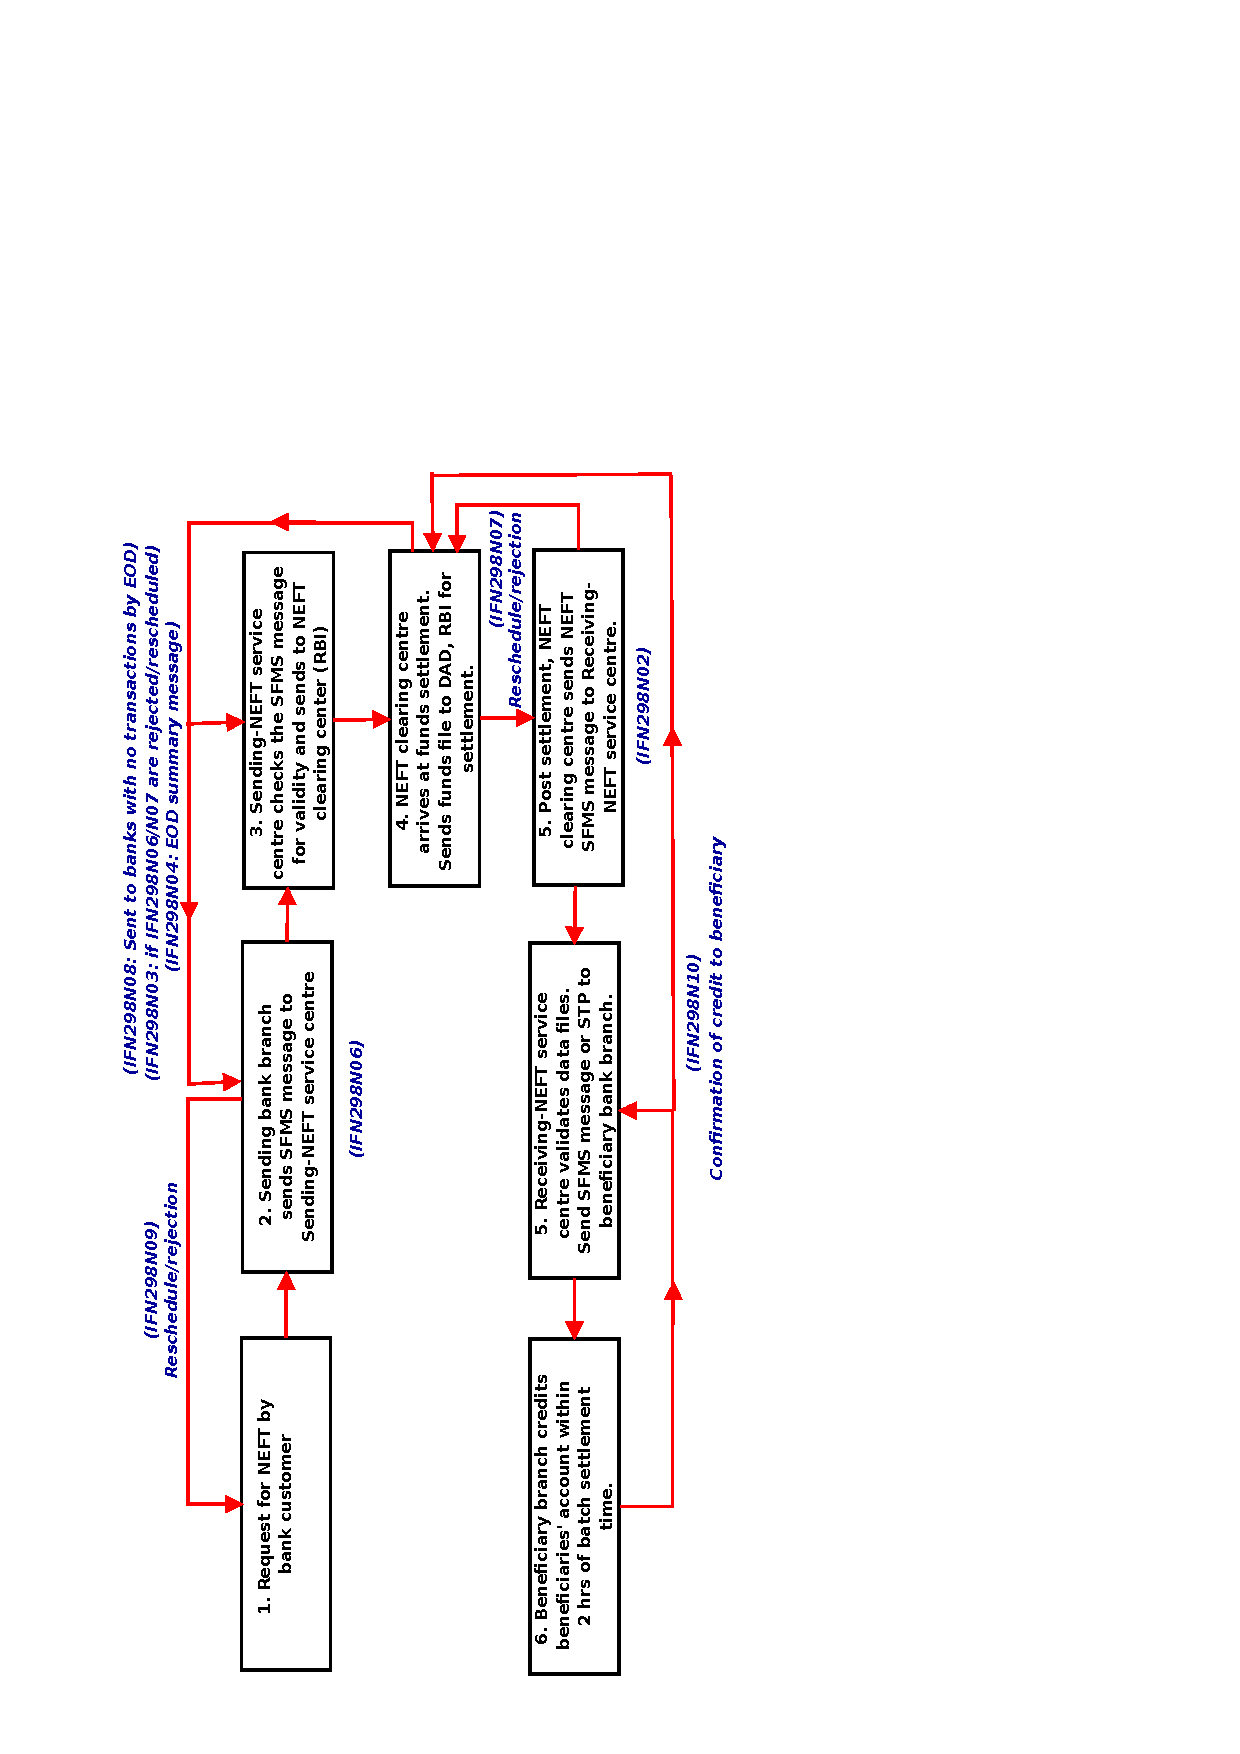
\includegraphics[scale = 0.5, angle = 270]{GRAPHS/neft_process_flow.pdf}
    \end{center}
  \end{figure}
\end{frame}

\fullpage{Data details}

\begin{frame}
  \frametitle{Introduction}
  \begin{footnotesize}
    \bf{Three major data sets:} 
    \begin{itemize}
      \begin{footnotesize}
      \item Location of RBI's currency chests
      \item Data on digital transactions
      \item Other data
      \end{footnotesize}
    \end{itemize}
  \end{footnotesize}
\end{frame}

\begin{frame}
  \frametitle{Location of RBI's currency chests}
  \begin{footnotesize}
    \begin{itemize}
    \item Total no. of RBI's currency chests: 4,040
    \item Total no. of unique pincode locations for currency chests: 2,915
    \item Out of 2,915 unique pincode locations:
      \begin{itemize}
      \item 2,840 pincodes: clean observations 
      \item 75 pincodes: junk, typo errors in pincodes (collected-manually)
      \end{itemize}
    \item \textbf{The final data base for currency chests includes pincodes for all 4,040 chests. These are exclusive of the chests in Panaji.}  
    \end{itemize}
  \end{footnotesize}
\end{frame}

\begin{frame}
  \frametitle{Location of RBI's currency chests (4,040 chests)}
  \begin{figure}
    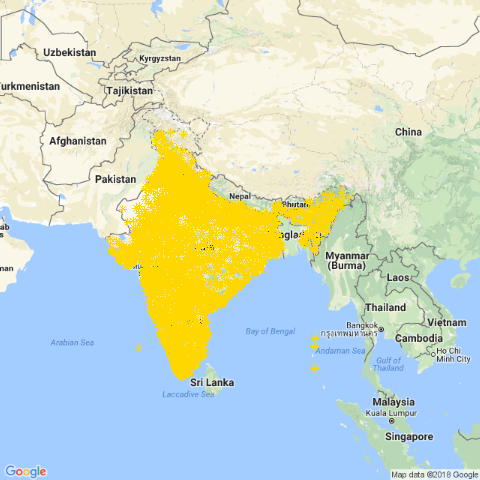
\includegraphics[scale = 0.45]{GRAPHS/india_cc_map.png}
  \end{figure}
\end{frame}

\begin{frame}[fragile]
  \frametitle{Location of RBI's currency chests (Data snapshot)}
  \begin{footnotesize}

    
\begin{knitrout}
\definecolor{shadecolor}{rgb}{0.969, 0.969, 0.969}\color{fgcolor}\begin{kframe}
\begin{alltt}
\hlkwd{load}\hlstd{(}\hlstr{'../SRC/DATA/complete_data_cc.rda'}\hlstd{,} \hlkwc{verbose} \hlstd{=} \hlnum{TRUE}\hlstd{)}
\end{alltt}
\begin{verbatim}
## Loading objects:
##   cc_with_latlon
\end{verbatim}
\begin{alltt}
\hlkwd{head}\hlstd{(cc_with_latlon,} \hlnum{9}\hlstd{)}
\end{alltt}
\begin{verbatim}
##           cc_branch district        state pin_code      lat      lon
## 1 Parliament Street    DELHI NCT OF DELHI   110001 28.63274 77.21960
## 2 Parliament Street    DELHI NCT OF DELHI   110001 28.63274 77.21960
## 3 Parliament Street    DELHI NCT OF DELHI   110001 28.63274 77.21960
## 4 Parliament Street    DELHI NCT OF DELHI   110001 28.63274 77.21960
## 5 Parliament Street    DELHI NCT OF DELHI   110001 28.63274 77.21960
## 6    Shastri Bhawan    DELHI NCT OF DELHI   110001 28.63274 77.21960
## 7 Parliament Street    DELHI NCT OF DELHI   110001 28.63274 77.21960
## 8     Lawrence Road    DELHI NCT OF DELHI   110035 28.67383 77.16426
## 9          Inderlok    DELHI NCT OF DELHI   110035 28.67383 77.16426
\end{verbatim}
\end{kframe}
\end{knitrout}
  \end{footnotesize}
\end{frame}

\begin{frame}
  \frametitle{Data on digital transactions}
  \begin{footnotesize}
    \textbf{Databases}:
    \begin{enumerate}
    \item RuPay credit card (POS and e-commerce transactions) (NPCI)
    \item NEFT (RBI)
    \item RTGS (RBI)
    \item Mobile transactions (RBI)
    \end{enumerate}
    \vspace{7mm}
    \textbf{Geo-coding of transactions} data will be done using either:
    \begin{enumerate}
    \item Direct mapping for pincodes or
    \item Indirect mapping for pincodes using IFSC codes
    \end{enumerate}
  \end{footnotesize}
\end{frame}

\begin{frame}
  \frametitle{Data on digital transactions: Direct mapping for pincodes}
  \begin{footnotesize}
    \textbf{India's complete pincodes directory}
    \begin{itemize}
    \item Total no. of unique locations: 154,797
    \item Total no. of unique pincodes: 19,100
    \item Out of 19,100 unique pincodes:
      \begin{enumerate}
      \item 18,867 pincodes: clean observations (153,250 locations)
      \item 233 pincodes: junk, typo errors or pincode does not exist anymore 
      \end{enumerate}
    \end{itemize}
  \end{footnotesize}
\end{frame}

\begin{frame}
  \frametitle{Data on digital transactions: Direct mapping for pincodes (18,867 pincodes)}
  \begin{figure}
    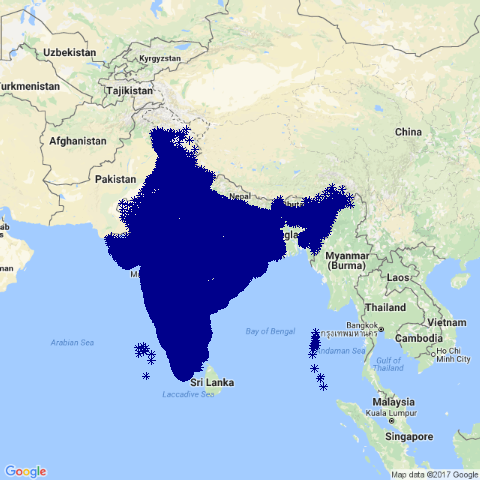
\includegraphics[scale = 0.45]{GRAPHS/india_pin_map.png}
  \end{figure}
\end{frame}

\begin{frame}[fragile]
  \frametitle{Data on digital transactions: Direct mapping for pincodes (Data snapshot)}
  \begin{footnotesize}
\begin{knitrout}
\definecolor{shadecolor}{rgb}{0.969, 0.969, 0.969}\color{fgcolor}\begin{kframe}
\begin{alltt}
\hlkwd{load}\hlstd{(}\hlstr{'../SRC/DATA/complete_data_pin_dir.rda'}\hlstd{,} \hlkwc{verbose} \hlstd{=} \hlnum{TRUE}\hlstd{)}
\end{alltt}
\begin{verbatim}
## Loading objects:
##   pin_dir_with_latlon
\end{verbatim}
\begin{alltt}
\hlkwd{head}\hlstd{(pin_dir_with_latlon,} \hlnum{9}\hlstd{)}
\end{alltt}
\begin{verbatim}
##   pincode talukname districtname statename      lat      lon
## 1  504273  Asifabad     Adilabad TELANGANA 19.22441 79.60529
## 2  504273  Asifabad     Adilabad TELANGANA 19.22441 79.60529
## 3  504273  Asifabad     Adilabad TELANGANA 19.22441 79.60529
## 4  504273  Asifabad     Adilabad TELANGANA 19.22441 79.60529
## 5  504273  Asifabad     Adilabad TELANGANA 19.22441 79.60529
## 6  504273  Asifabad     Adilabad TELANGANA 19.22441 79.60529
## 7  504273  Asifabad     Adilabad TELANGANA 19.22441 79.60529
## 8  504273  Asifabad     Adilabad TELANGANA 19.22441 79.60529
## 9  504273  Asifabad     Adilabad TELANGANA 19.22441 79.60529
\end{verbatim}
\end{kframe}
\end{knitrout}
  \end{footnotesize}
\end{frame}

\begin{frame}
  \frametitle{Data on digital transactions: Indirect mapping of pincodes using IFSC}
  \begin{footnotesize}
    Quality of IFSC database available on web is poor.
    \begin{itemize}
    \item Total no. of banks: \textbf{196} (List of branches available for \textbf{195})
    \item Total no. of bank branches: \textbf{151,921} 
      \begin{enumerate}
      \item Valid 11-digit IFSC codes available for \textbf{138,376}.
      \item Valid pincodes available for \textbf{96,134}.
        \begin{itemize}
        \item Junk values due to typographical errors are possible.
        \item No. of unique pincodes in IFSC database are 19,120 while in India's directory it is 19,100 (?)  
        \end{itemize}
      \end{enumerate}  
    \end{itemize}
  \end{footnotesize}
\end{frame}

\begin{frame}
  \frametitle{Other data}
  \begin{enumerate}
    \begin{footnotesize}
    \item Location of mobile towers across the country
    \item Quality of mobile calls
    \item Availability of 3G networks in an area
    \item Number of subscribers
    \item Mobile coverage
    \item Mobile penetration data
    \item Credit card data (CMIE consumer pyramids)
    \item Bank account penetration data (CMIE consumer pyramids)
    \item 2011 census data (city demographics, average education, percentage of salaried vs self-employed)
    \item 2013 NSSO data (Formal vs informal employment)
    \end{footnotesize}
  \end{enumerate}
\end{frame}


\begin{frame}
  \begin{center}
    Thank you.
    \vspace{0.1in}
  \end{center}
\end{frame}


\end{document}

